\section{Proposed Method}
\label{sec:proposed}

\subsection{Adversarially Robust Autoencoder}
\label{sec:proposed_inversion}

We propose an autoencoder architecture (\figref{fig:proposed_model}) to extract bottleneck AR features of arbitrary input images, manipulate them for a given synthesis task, and map the results back to images. We denote the AR feature extractor as $F_{\tilde{\theta}}$, where $\tilde{\theta}$ are the AR model weights, as explained in \secref{sec:framework}. Robust features are transformed into images using a CNN-based generator denoted as $G_{\tilde{\phi}}$. Here, $\tilde{\phi}$ are the generator weights learned by inverting AR features.

Following prior works~\cite{ulyanov2018deep,dosovitskiy_2016_generating}, we use AlexNet as the encoder and extract AR features from its \layer{conv5} layer. We also explore more complex encoders from the VGG and ResNet families and evaluate their improvement over standard encoders (See \secref{sec:supp_proposed} for architecture details).

\begin{figure}[t]
\hspace{0.55\textwidth}\begin{minipage}{0.15\textwidth}
\centering \textbf{\colorbox{white}{\scalebox{.7}{Ground-truth}}}
\end{minipage}\begin{minipage}{0.15\textwidth}
\centering \textbf{\colorbox{white}{\scalebox{.7}{Standard}}}
\end{minipage}\begin{minipage}{0.15\textwidth}
\centering \textbf{\colorbox{white}{\scalebox{.7}{AR (ours)}}}
\end{minipage}

\vspace{-0.9 cm}
\subfloat[Proposed Adversarially Robust Model]{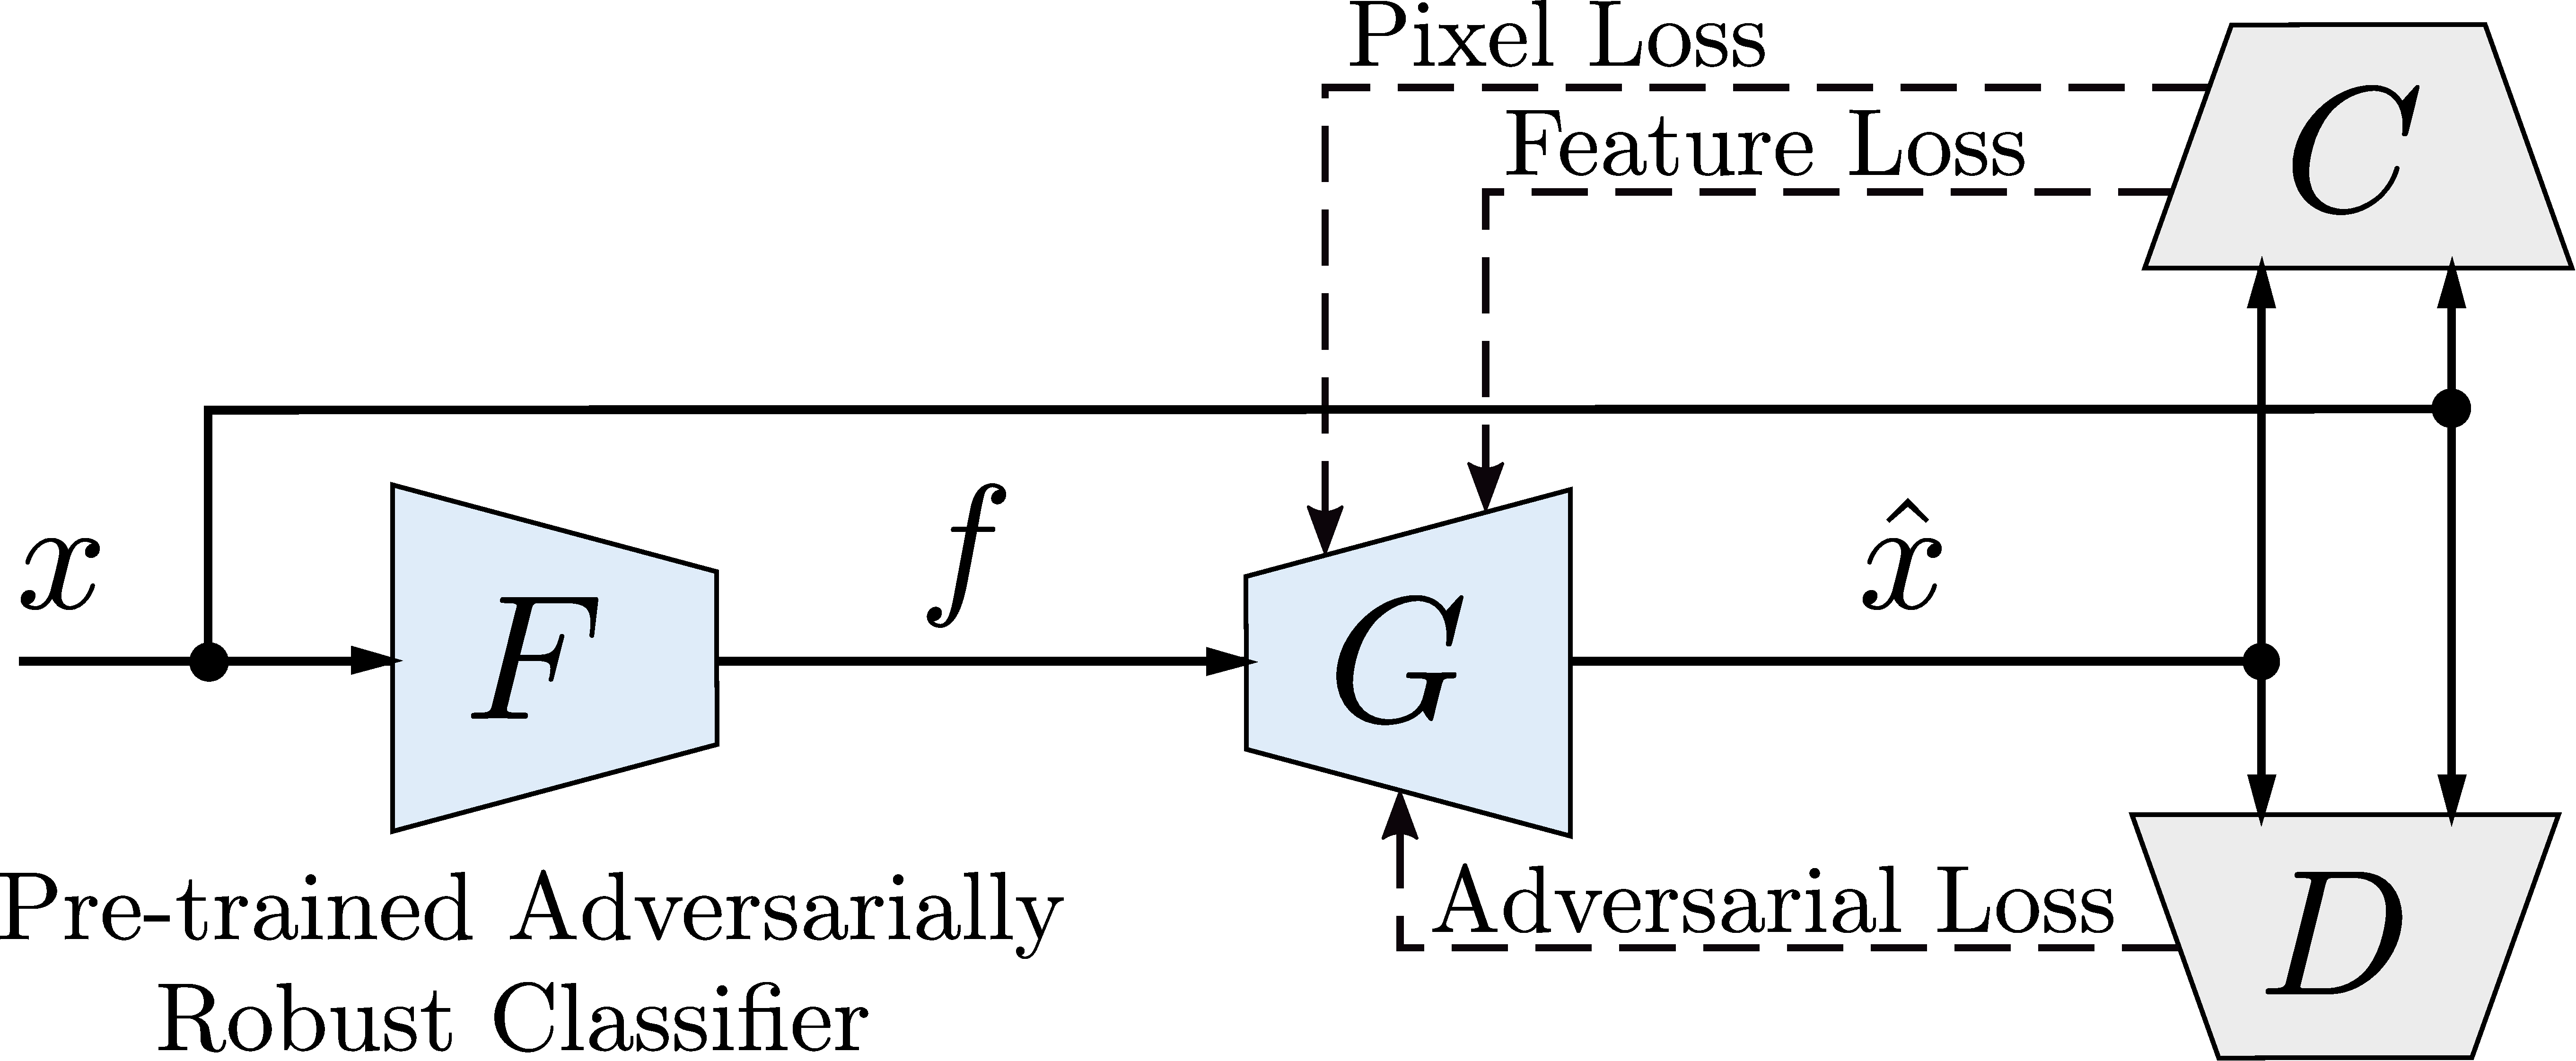
\includegraphics[width=0.45\textwidth]{figs/proposed/encdec.pdf}\hspace{0.1\textwidth}}
\subfloat[Feature Inversion ($224 \times 224$ px.)]{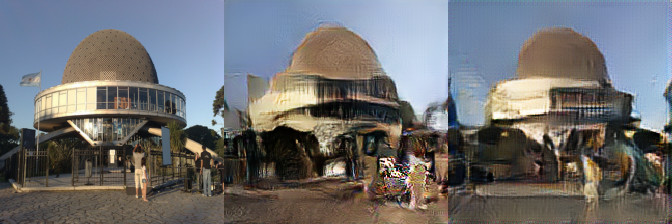
\includegraphics[width=0.45\textwidth]{figs/lowres/tile_inversion.jpg}}


\caption{\label{fig:proposed_model}By training it to invert adversarially robust features, our proposed autoencoder obtains better reconstructions than models trained on standard features.}
\vspace{-0.5cm}
\end{figure}


\subsection{Image Decoder: Optimization Criteria}
\label{sec:opt_crit}

Given a pre-trained AR encoder $F_{\tilde{\theta}}$, the generator $G_{\tilde{\phi}}$ is trained using $\ell_{1}$ pixel, $\ell_{2}$ feature and GAN losses, where the feature loss matches AR representations, known to be \textit{perceptually aligned} \cite{engstrom_2019_adversarial}.

In more detail, we denote $\hat{x}=G_{\tilde{\phi}}(f)$ to be the reconstruction of image $x$, where $f=F_{\tilde{\theta}}(x)$ are its AR features. Training the generator with fixed encoder's weights $\tilde{\theta}$  corresponds to the following optimization problem:
\begin{align}
    \tilde{\phi}=\ \text{arg }\underset{\phi}{\text{min}}&\ \lambda_{\text{pix}}\mathcal{L}_{\text{pix}}(\phi)+\lambda_{\text{feat}}\mathcal{L}_{\text{feat}}(\phi, \tilde{\theta}) + \lambda_{\text{adv}}\mathcal{L}_{\text{adv}}(\phi,\psi),
\end{align}
\vspace{-1.5\baselineskip}
\begin{align}
    \mathcal{L}_{\text{pix}}(\phi)\triangleq& \ \mathbb{E}_{x\sim \tilde{\mathcal{K}}}\ \|x-G_{\phi}(f)\|_{1},\\
    \mathcal{L}_{\text{feat}}(\phi, \tilde{\theta})\triangleq& \ \mathbb{E}_{x\sim \tilde{\mathcal{K}}}\ \|f-F_{\tilde{\theta}}\circ G_{\phi}(f)\|_{2}^{2},\\
    \mathcal{L}_{\text{adv}}(\phi, \psi)\triangleq&\ \mathbb{E}_{x\sim \tilde{\mathcal{K}}}\big[-\text{log}D_{\psi}\circ G_{\phi}(f)\big],
\end{align}
where $\lambda_{\text{pix}}, \lambda_{\text{feat}}, \lambda_{\text{adv}}\in \R_{++}$ are hyperparameters,  $D_{\psi}: \R^{W \times H \times C}\mapsto [0,1]$ denotes the discriminator with weights $\psi$ and predicts the probability of an image being real.
The pixel loss $\mathcal{L}_{\text{pix}}(\phi)$ is the $\ell_{1}$ distance between prediction $G_{\phi}(f)$ and target $x$. The feature loss $\mathcal{L}_{\text{feat}}(\phi, \theta)$ is the $\ell_{2}$ distance between the AR features of prediction and target. The adversarial loss $\mathcal{L}_{\text{adv}}(\phi, \psi)$ maximizes the discriminator score of predictions, \ie, it increases the chance the discriminator classifies them as real. On the other hand, the discriminator weights are trained via the cross-entropy loss, \ie, 
\begin{align}
 \min_\psi \mathcal{L}_{\text{disc}}(\phi, \psi)\triangleq&\ \mathbb{E}_{x\sim \tilde{\mathcal{K}}}\big[-\text{log}D_{\psi}(x)-\text{log}(1-D_{\psi}\circ G_{\phi}(f))\big].
\end{align}
This discriminative loss $ \mathcal{L}_{\text{disc}}(\phi, \psi)$ guides $D_\psi$ to maximize the score of real images and minimize the score of reconstructed (fake) images. Similar to traditional GAN algorithms, we alternate between the generator and discriminator training to reach the equilibrium point.

\subsection{Applications}
\label{sec:applications}

The trained AR autoencoder can be used to improve the performance of tasks such as style transfer \cite{li_2017_universal}, image denoising \cite{vincent_2010_stacked}, and anomaly detection \cite{deecke_2018_image}. In what follows, we describe the use of our model on style transfer and image denoising. The task of anomaly detection is covered in the Appendix (\secref{sec:supp_anomaly_detection}).

\textbf{Example-based Style Transfer.} Style transfer \cite{gatys_2016_image} aligns deep features to impose perceptual properties of a style image $x_{s}$ over semantic properties of a content image $x_{c}$. This is done by matching the content and style distributions in the latent space of a pre-trained encoder to then transform the resulting features back into images. We adopt the Universal Style Transfer framework \cite{li_2017_universal} to show the benefits of using our AR model for stylization (\figref{fig:proposed_st}).

\begin{figure}[t]
\hspace{0.5\textwidth}
\begin{minipage}{0.09\textwidth}
\centering\textbf{\scriptsize{Refs}}
\end{minipage}\begin{minipage}{0.225\textwidth}
\centering\textbf{\scriptsize{Standard}}
\end{minipage}\begin{minipage}{0.175\textwidth}
\centering\textbf{\scriptsize{AR (ours)}}
\end{minipage}\vspace{-2\baselineskip}

\subfloat[Multilevel Stylization]{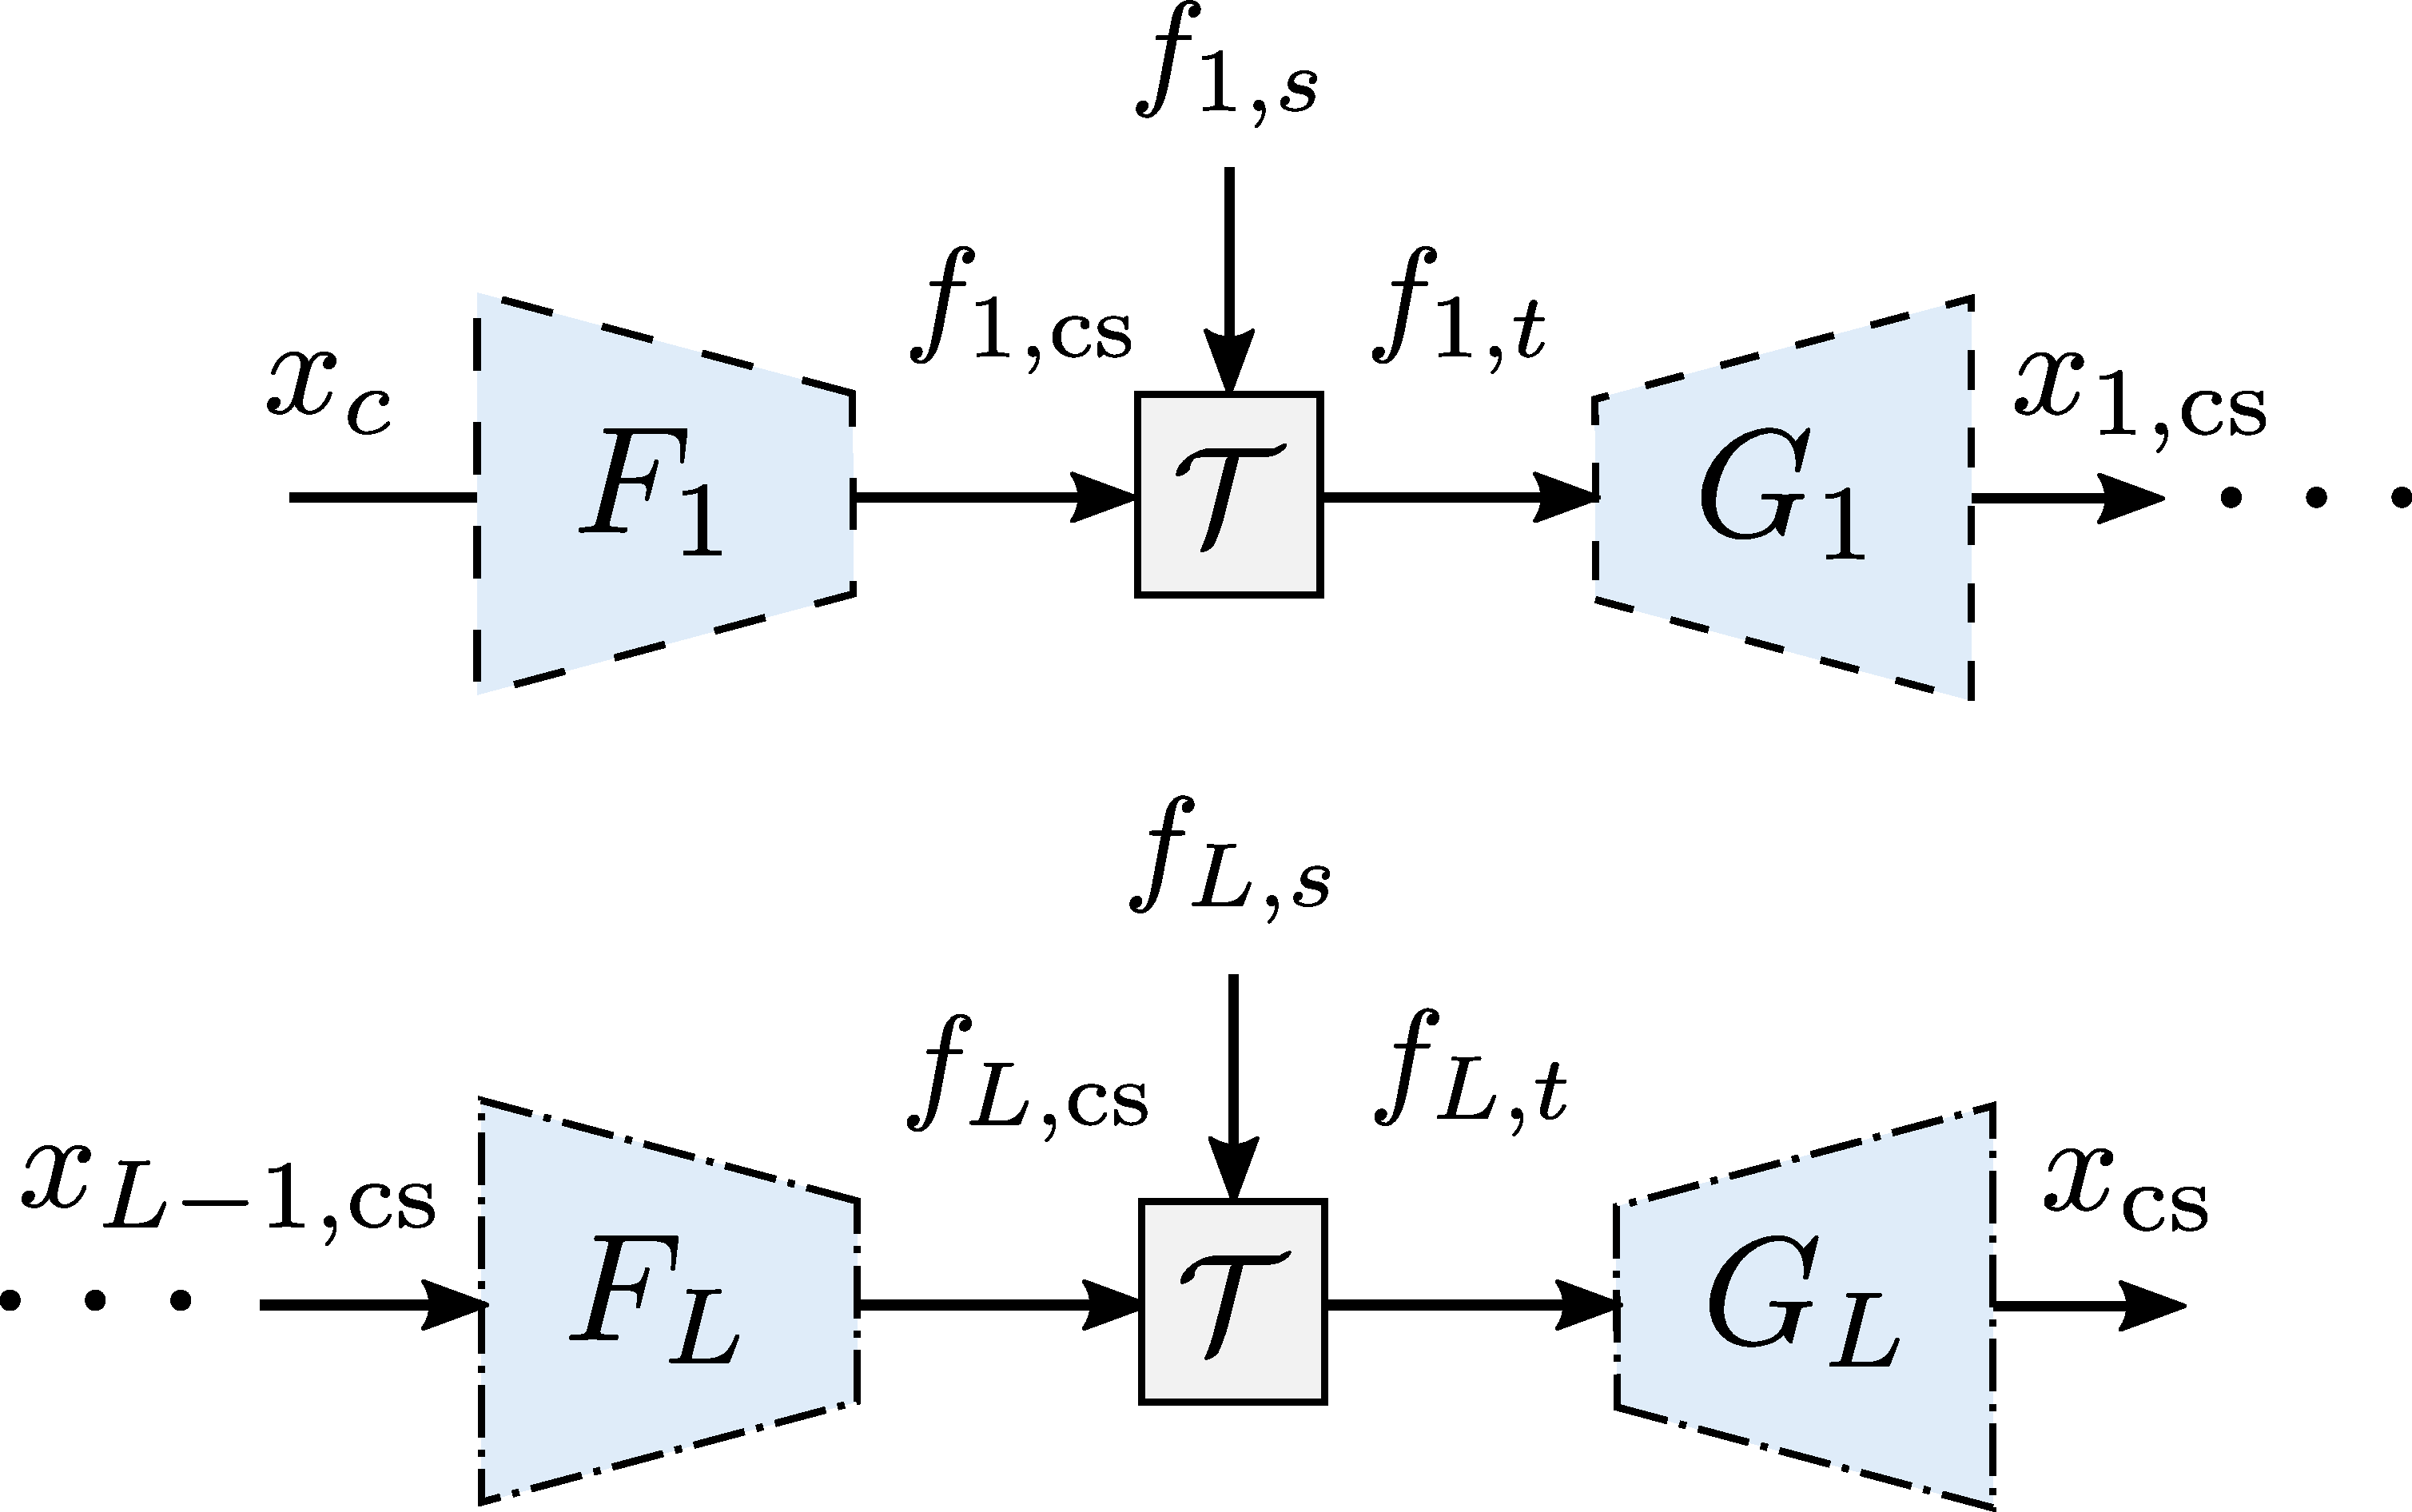
\includegraphics[width=0.375\textwidth]{figs/proposed/st_diag.pdf}}\hspace{0.125\textwidth}
\subfloat[Adversarially Robust Style Transfer]{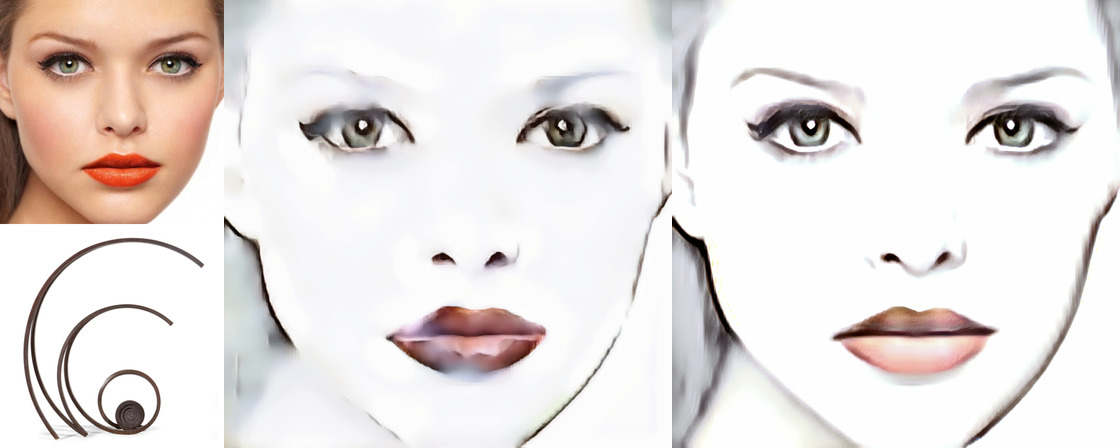
\includegraphics[width=0.5\textwidth]{figs/st/st_tile01.jpg}}

\vspace{-0.2cm}
\caption{\label{fig:proposed_st}Example-based Style Transfer using adversarially robust features.}
\vspace{-0.2cm}
\end{figure}

\begin{figure}[t]

\hspace{0.45\textwidth}
\begin{minipage}[t]{0.1375\textwidth}
\centering\textbf{\colorbox{white}{\scalebox{.7}{\hspace{-0.35\baselineskip}Ground-truth}}}
\end{minipage}\begin{minipage}[t]{0.1375\textwidth}
\centering \textbf{\colorbox{white}{\scalebox{.7}{Observation}}}
\end{minipage}\begin{minipage}[t]{0.1375\textwidth}
\centering \textbf{\colorbox{white}{\scalebox{.7}{Standard}}}
\end{minipage}\begin{minipage}[t]{0.1375\textwidth}
\centering \textbf{\colorbox{white}{\scalebox{.7}{AR (ours)}}}

\end{minipage}\vspace{-0.5 cm}
\subfloat[Skip connected AR model]{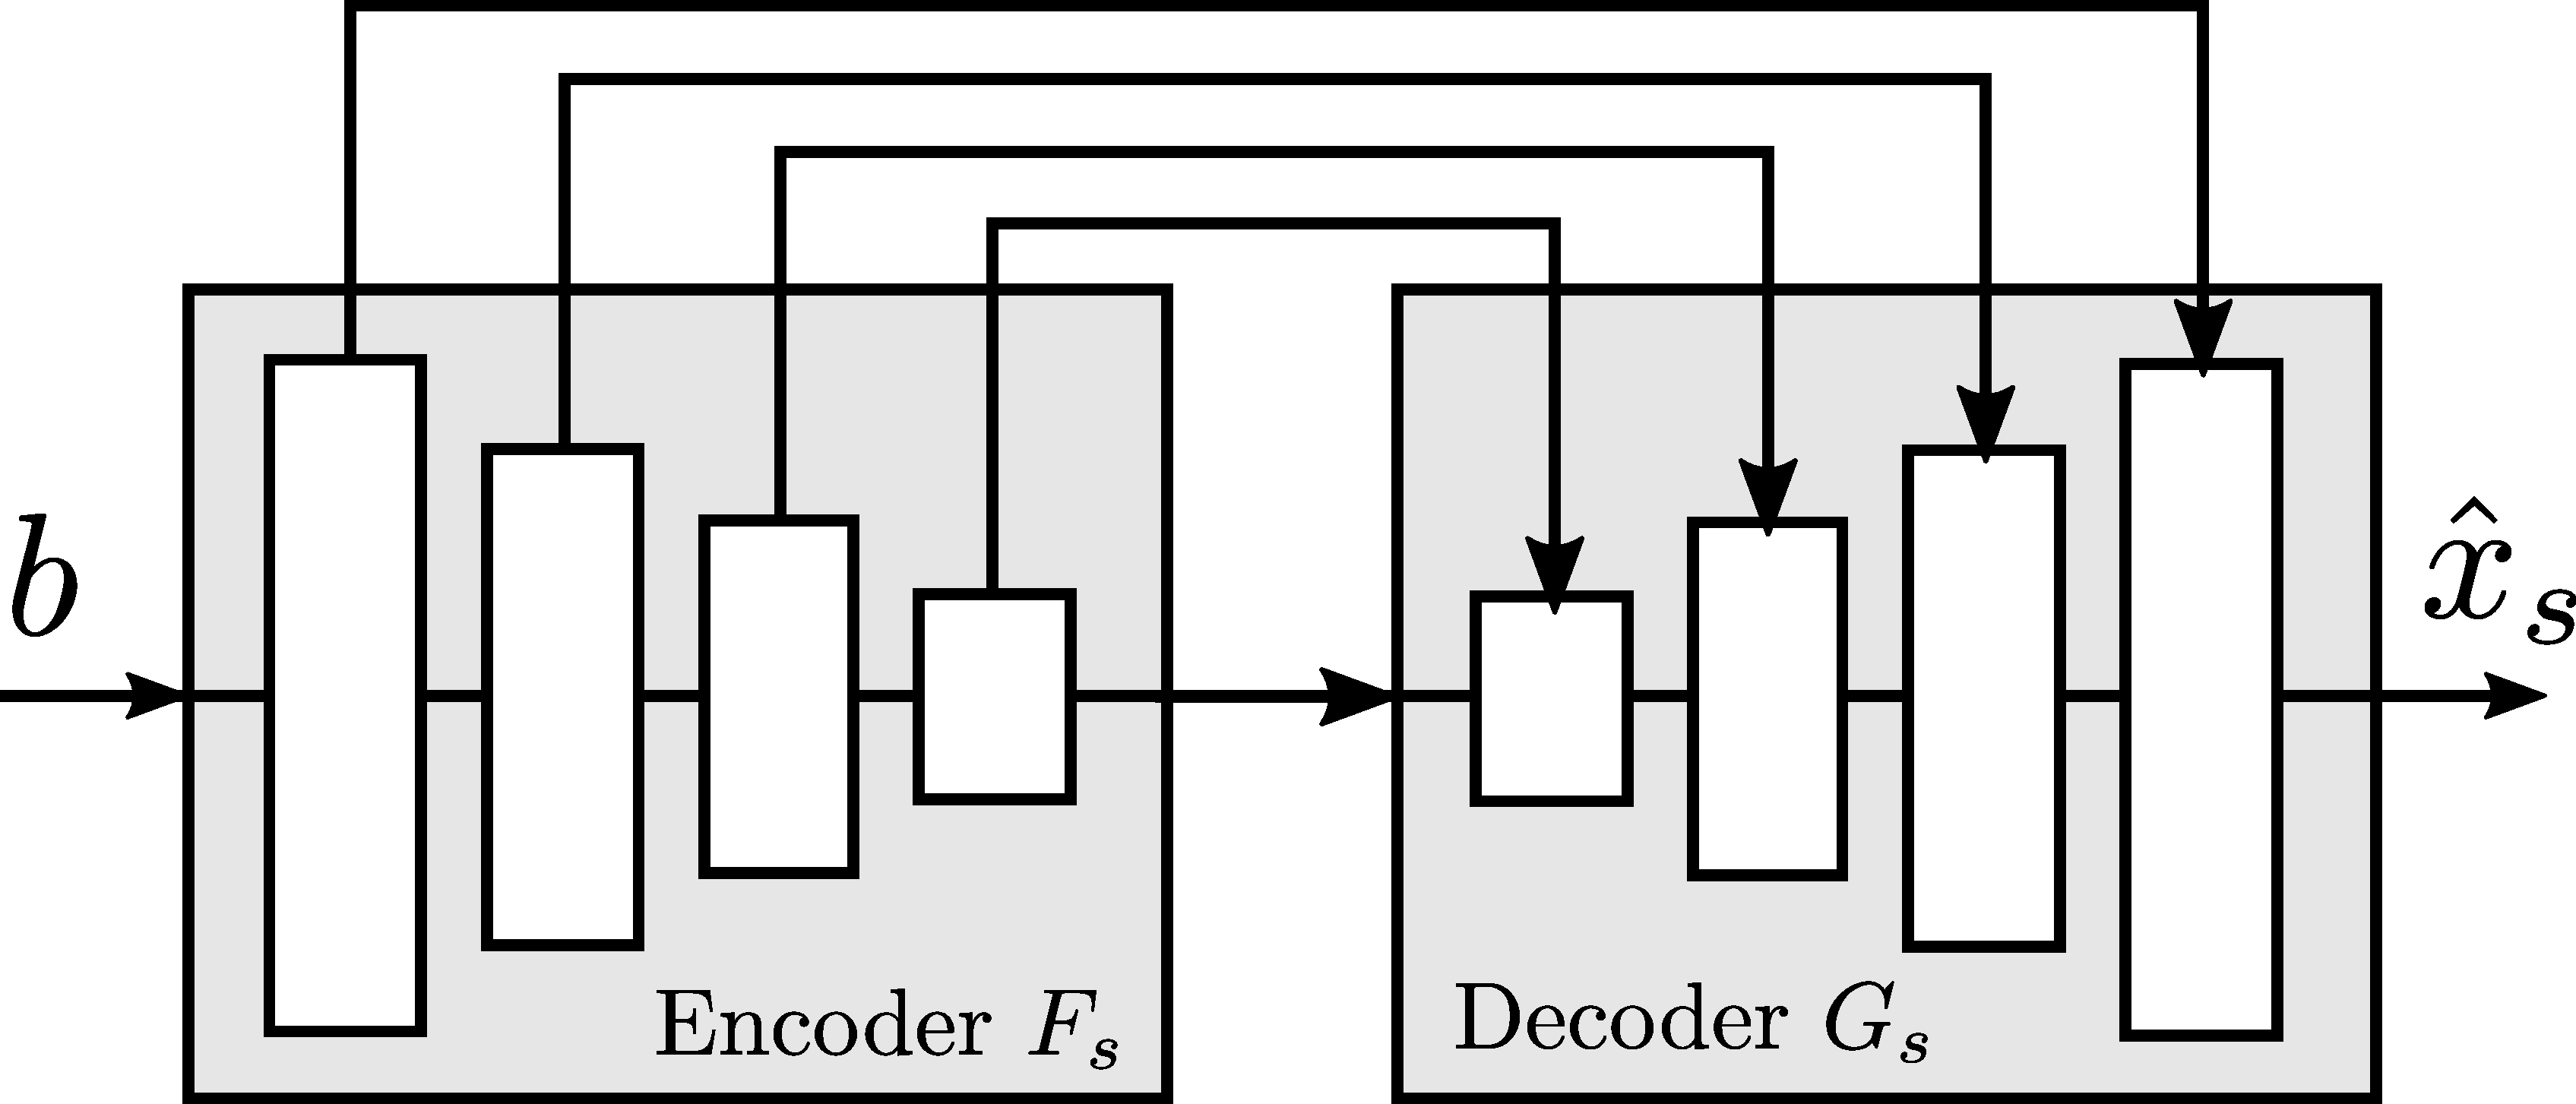
\includegraphics[width=0.4\textwidth]{figs/proposed/denoising_diag.pdf}}\hspace{0.05\textwidth}
\subfloat[Adversarially Robust Image Denoising]{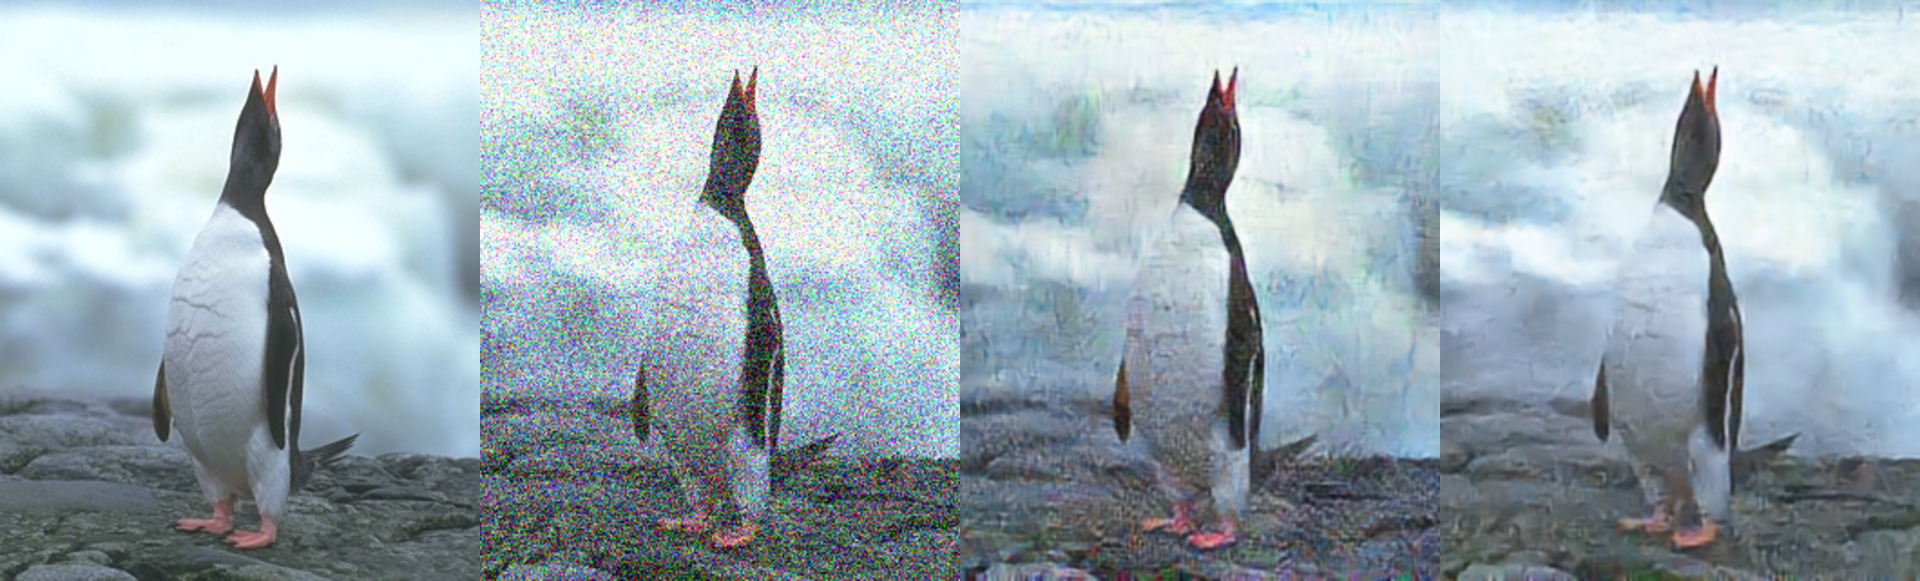
\includegraphics[width=0.55\textwidth]{figs/denoising/cbsd68_tile0.jpg}}

\vspace{-0.2 cm}
\caption{\label{fig:proposed_denoising}Image denoising using our adversarially robust autoencoder.}
\vspace{-0.7 cm}
\end{figure}


We train three AR AlexNet autoencoders $\{F_{l,\tilde{\theta}}, G_{l,\tilde{\phi}}\}_{l=1}^{L=3}$ and use them to sequentially align features at each scale. $F_{1,\tilde{\theta}}$, $F_{2,\tilde{\theta}}$ and $F_{3,\tilde{\theta}}$ extract AR \layer{conv5}, \layer{conv2} and \layer{conv1} features, respectively. First, style features $f_{l,s}=F_{l,\tilde{\theta}}(x_{s})$ are extracted at each stage. We then use the content image as initialization for the stylized output $x_{0,\text{cs}}\triangleq x_{c}$ and extract its \layer{conv5} features $f_{1,\text{cs}}=F_{1,\tilde{\theta}}(x_{0,\text{cs}})$.

At stage $l=1$, the style distribution is imposed over the content features by using the whitening and coloring transform \cite{li_2017_universal,kessy_2018_optimal} denoted by $\mathcal{T}$. The resulting representation $f_{1,t}= \mathcal{T}\big(f_{1,s},f_{1,\text{cs}}\big)$ is characterized by the first and second moments of the style distribution. An intermediate stylized image $x_{1,\text{cs}}$ incorporating the style at the first scale is then generated as $x_{1,\text{cs}}= G_{1,\tilde{\phi}}(f_{1,t})$.

The process is repeated for $l\in \{2,3\}$ to incorporate the style at finer resolutions, resulting in the final stylized image $x_{\text{cs}}= x_{3,\text{cs}}$.


\textbf{Image Denoising.} Motivated by denoising autoencoders (DAE) \cite{vincent_2010_stacked} where meaningful features are extracted from distorted instances, we leverage AR features for image enhancement tasks. Similarly to deep denoising models \cite{mao_2016_image}, we incorporate skip connections in our pre-trained AR AlexNet autoencoder to extract features at different scales, complementing the information distilled at the encoder bottleneck (\figref{fig:proposed_denoising}).
Skip connections correspond to Wavelet Pooling \cite{yoo_2019_photorealistic}, replacing pooling and upsampling layers by analysis and synthesis Haar wavelet operators, respectively. Our skip-connected model is denoted by $\{F_{s, \tilde{\theta}}, G_{s, \tilde{\phi}}\}$.

Similarly to real quantization scenarios \cite{el_2020_blind,zhang_2018_ffdnet,moeller_2015_learning}, we assume images are corrupted by clipped additive Gaussian noise. A noisy image is denoted by $b= \rho\big(x+\eta\big)\ \in \R^{W\times H\times C}$, where $\eta\sim \mathcal{N}(0, \sigma)$ is the additive white Gaussian noise term and $\rho(x)= \max[0, \min(1, x)]$ a pointwise operator restricting the range between $0$ and $1$. Denoised images are denoted by $\hat{x}_{s}= G_{s,\tilde{\phi}}\circ F_{s,\tilde{\theta}}(b)$.

$G_{s, \tilde{\phi}}$ is trained to recover an image $x$ from the features of its corrupted version $F_{s, \tilde{\theta}}(b)$. The training process uses the optimization criteria described in \secref{sec:opt_crit}.
